\documentclass[CJK]{beamer}
\usepackage{CJKutf8}
\usepackage{beamerthemesplit}
\usetheme{Malmoe}
\useoutertheme[footline=authortitle]{miniframes}
\usepackage{amsmath}
\usepackage{amssymb}
\usepackage{graphicx}
\usepackage{color}
\usepackage{slashed}
\usepackage{simplewick}
\graphicspath{{../figures/}}
\def\be{\begin{equation}}
\def\ee{\nonumber\end{equation}}
\def\bea{\begin{eqnarray}}
\def\eea{\nonumber\end{eqnarray}}
\def\ii{{\dot{\imath}}}
\def\bch{\begin{CJK}{UTF8}{gbsn}}
\def\ech{\end{CJK}}
\def\bex{\begin{minipage}{0.3\textwidth}
\includegraphics[width=1in]{jugelizi.png}\end{minipage}\begin{minipage}{0.6\textwidth}}
\def\eex{\end{minipage}}
\def\chtitle#1{\frametitle{\bch#1\ech}}
\def\skipline{{\vskip0.1in}}
\def\skiplines{{\vskip0.2in}}
\def\lagr{{\mathcal{L}}}
\def\hamil{{\mathcal{H}}}
\def\vecv{{\mathbf{v}}}
\def\vecx{{\mathbf{x}}}
\def\veck{{\mathbf{k}}}
\def\vecp{{\mathbf{p}}}
\def\vecn{{\mathbf{n}}}
\def\vecA{{\mathbf{A}}}
\def\vecP{{\mathbf{P}}}
\def\vecsigma{{\mathbf{\sigma}}}
\def\hatJn{{\hat{J_\vecn}}}
\def\hatJx{{\hat{J_x}}}
\def\hatJy{{\hat{J_y}}}
\def\hatJz{{\hat{J_z}}}
\def\hatj#1{\hat{J_{#1}}}
\def\hatphi{{\hat{\phi}}}
\def\hatq{{\hat{q}}}
\def\hatpi{{\hat{\pi}}}
\def\vel{\upsilon}
\def\Dint{{\mathcal{D}}}
\def\adag{{\hat{a}^\dagger}}
\def\bdag{{\hat{b}^\dagger}}
\def\cdag{{\hat{c}^\dagger}}
\def\ddag{{\hat{d}^\dagger}}
\def\hata{{\hat{a}}}
\def\hatb{{\hat{b}}}
\def\hatc{{\hat{c}}}
\def\hatd{{\hat{d}}}
\def\hatN{{\hat{N}}}
\def\hatH{{\hat{H}}}
\def\hatp{{\hat{p}}}
\def\Fup{{F^{\mu\nu}}}
\def\Fdown{{F_{\mu\nu}}}
\def\newl{\nonumber \\}
\def\SIkm{\mathrm{km}}
\def\SIyr{\mathrm{yr}}
\def\SIGyr{\mathrm{Gyr}}
\def\SIeV{\mathrm{eV}}
\def\SIGeV{\mathrm{GeV}}
\def\SIm{\mathrm{m}}
\def\SIcm{\mathrm{cm}}
\def\SIJ{\mathrm{J}}
\def\SIs{\mathrm{s}}
\def\SIkg{\mathrm{kg}}
\def\SIg{\mathrm{g}}
\def\vece{\mathrm{e}}
\def\bmat#1{\left(\begin{array}{#1}}
\def\emat{\end{array}\right)}
\def\bcase#1{\left\{\begin{array}{#1}}
\def\ecase{\end{array}\right.}
\def\calM{{\mathcal{M}}}
\def\calT{{\mathcal{T}}}
\def\calR{{\mathcal{R}}}
\def\barpsi{\bar{\psi}}
\def\baru{\bar{u}}
\def\barv{\bar{\upsilon}}
\def\bmini#1{\begin{minipage}{#1\textwidth}}
\def\emini{\end{minipage}}
\def\qeq{\stackrel{?}{=}}
\def\torder#1{\mathcal{T}\left(#1\right)}
\def\rorder#1{\mathcal{R}\left(#1\right)}


\title{Quantum Field Theory I \\ Lesson 10 - Quantization of Spinors}
\author{}
\date{}


\begin{document}

\begin{frame}
 
\begin{center}
\begin{Large}
\bch
量子场论 I 

{\vskip 0.3in}

第十课 旋量场的量子化

\ech
\end{Large}
\end{center}

\vskip 0.2in

\bch
课件下载
\ech
https://github.com/zqhuang/SYSU\_QFTI

\end{frame}


\begin{frame}
\chtitle{Dirac方程的解的性质}
\bch
我们上节课得到了Dirac方程的经典解,如果定义
$$\theta_{\veck,s}  \equiv 2s\tan^{-1}\frac{\omega - m}{|\veck|} = 2s\tan^{-1}\frac{|\veck|}{\omega+m}$$
\be
 u_{\veck,s} = 
\bmat{c}
\zeta_{\veck,s} \cos\theta_{\veck,s} \\
\zeta_{\veck,s} \sin\theta_{\veck,s}
\emat
\ee
\be
 \upsilon_{\veck,s} = 
\bmat{c}
\zeta_{\veck,s} \sin\theta_{\veck,s} \\
-\zeta_{\veck,s} \cos\theta_{\veck,s}
\emat
\ee
容易验证$u_{\veck,s}e^{-\ii\omega t}$和$\upsilon_{\veck,s}e^{\ii\omega t}$就是我们上节课推导的Dirac方程的对应于$k_0 = \pm \omega$的解。
\ech
\end{frame}


\begin{frame}
\chtitle{Dirac方程的解的性质}
\bch
利用自旋本征态的正交归一条件:$\zeta^\dagger_{\veck,s}\zeta_{\veck,s'}=\delta_{ss'}$,可以证明:
\bea
u_{\veck,s}^\dagger u_{\veck,s'} &=&  \upsilon_{\veck,s}^\dagger \upsilon_{\veck,s'} = \delta_{ss'} \newl
u_{\veck,s}^\dagger \upsilon_{\veck,s'} &=&  \upsilon_{\veck,s}^\dagger u_{\veck,s'} = 0 \newl
\bar{u}_{\veck,s} u_{\veck,s'} &=& \delta_{ss'}\cos{2\theta_{\veck,s}} \newl
\bar{\upsilon}_{\veck,s} \upsilon_{\veck,s'} &=& -\delta_{ss'}\cos{2\theta_{\veck,s}} \newl
\bar{u}_{\veck,s} \upsilon_{\veck,s'} &=&  \bar{\upsilon}_{\veck,s} u_{\veck,s'} = \delta_{ss'}\sin{2\theta_{\veck,s}} 
\eea
注意根据$\theta_{\veck,s}$的定义可以推出
$$\cos{2\theta_{\veck,s}} = m/\omega,\, \ \sin{2\theta_{\veck,s}} = |\veck|/\omega$$
\ech
\end{frame}

\begin{frame}
\chtitle{广义动量和Hamilton密度}
\bch

对应于$\psi$的广义动量为
$$\pi = \frac{\partial \lagr}{\partial (\dot\psi)} =\ii \psi^\dagger$$
于是
$$\hamil =\pi \dot\psi - \lagr = -\bar\psi(\ii\gamma^j\partial_j - m)\psi = \pi \gamma^0 ( -\gamma^j \partial_j - \ii m)\psi  $$
显然,满足Dirac方程的解$\psi$使得$\lagr = 0$。从而
$$\hamil = \pi\dot\psi = \ii \psi^\dagger \dot\psi$$

\ech
\end{frame}

\begin{frame}
\chtitle{其他守恒量}
\bch
利用时空平移对称性,可以求出四维动量密度为
$$P^\mu = \ii\psi^\dagger \partial^\mu \psi$$
显然$P^0 = \hamil$.

再利用规范对称性($\psi \rightarrow \psi e^{-iq\epsilon}$)可以得到守恒流为
$$j^\mu = q \bar\psi \gamma^\mu \psi$$
守恒荷密度
$$j^0 =  q\psi^\dagger\psi$$
\ech
\end{frame}


\begin{frame}
\chtitle{旋量场的量子化}
\bch
我们先把傅立叶空间的一般解写为:
$$\hat\psi_{\veck} = \sum_{s}\frac{u_{\veck,s}e^{-\ii \omega t} \hata_{\veck,s}|_{t=0} + \upsilon_{\veck,s}e^{\ii \omega t} \bdag_{-\veck,s}|_{t=0}}{\sqrt{d^3\veck}}$$
其中$\hata_{\veck,s}$和$\bdag_{-\veck,s}$为$t=0$时刻的待定算符。
我们也可以把时间演化因子吸收到算符里
$$\hat\psi_{\veck} = \sum_{s}\frac{u_{\veck,s} \hata_{\veck,s} + \upsilon_{\veck,s} \bdag_{-\veck,s}}{\sqrt{d^3\veck}}$$
任意时刻的$\hata_{\veck,s}$和$\bdag_{-\veck,s}$由下面的微分方程决定:
$$\frac{d\hata_{\veck,s}}{dt} = - \ii\omega \hata_{\veck,s},\ \ \ \frac{d\bdag_{-\veck,s}}{dt} = \ii\omega \bdag_{-\veck,s}$$
\ech
\end{frame}

\begin{frame}
\chtitle{旋量场的量子化}
\bch
从$\hat\psi$的表达式可以直接得到
$$\hat\psi^\dagger_{\veck} = \sum_s \frac{u^\dagger_{\veck,s} \adag_{\veck,s} + \upsilon^\dagger_{\veck,s} \hatb_{-\veck,s}}{\sqrt{d^3\veck}}$$
$$\ii \dot{\hat\psi}_{\veck} = \sum_s \omega  \frac{u_{\veck,s}\hata_{\veck,s} - \upsilon_{\veck,s}\bdag_{-\veck,s}}{\sqrt{d^3\veck}} $$
迄今为止,我们对算符$\hata$和$\hatb$只知道它们的时间演化规律。下面我们来尝试了解它们更多的性质。
\ech
\end{frame}

\begin{frame}
\chtitle{课堂讨论}
\bch
利用$u$,$\upsilon$的正交归一关系,证明Hamilton量为
$$\hat{H}_{\veck,s} =  \omega\left(\adag_{\veck,s}\hata_{\veck,s} - \hatb_{-\veck,s}\bdag_{-\veck,s} \right)$$
三维动量为
$$\hat{\mathbf{P}}_{\veck,s} =  \veck\left(\adag_{\veck,s}\hata_{\veck,s} + \hatb_{-\veck,s}\bdag_{-\veck,s} \right)$$
守恒荷为
$$\hat{Q}_{\veck,s} =  q\left(\adag_{\veck,s}\hata_{\veck,s} + \hatb_{-\veck,s}\bdag_{-\veck,s} \right)$$
\ech
\end{frame}

\begin{frame}
\chtitle{课堂讨论}
\bch
假设已知$[\hata_{\veck,s},\hatb_{-\veck,s}\bdag_{-\veck,s}]=[\adag_{\veck,s},\hatb_{-\veck,s}\bdag_{-\veck,s}]=0$, 证明

\begin{itemize}
\item{“粒子数算符”$\adag_{\veck,s}\hata_{\veck,s}$的本征值是非负实数}
\item{若把$\adag_{\veck,s}\hata_{\veck,s}$本征值为$n$的本征态记作$|n\rangle$,则$\hata_{\veck,s}|n\rangle = \sqrt{n}|n-1\rangle$}
\item{$\adag_{\veck,s}\hata_{\veck,s}$的本征值谱是连续的正整数$0,\, 1,\, 2,\, \ldots$。}
\item{若存在$|n+1\rangle$,则$\adag_{\veck,s}|n\rangle = \sqrt{n+1}|n+1\rangle$。若不存在$|n+1\rangle$,则$\adag_{\veck,s}|n\rangle =0$}
\end{itemize}

\skipline

提示:利用$\hata_{\veck,s}$的时间演化性质和海森堡方程。
\ech
\end{frame}


\begin{frame}
\chtitle{课堂讨论}
\bch
假设已知$[\adag_{\veck,s}\hata_{\veck,s},\bdag_{-\veck,s}]=[\adag_{\veck,s}\hata_{\veck,s},\hatb_{-\veck,s}]=0$, 证明

\begin{itemize}
\item{“空穴数算符”$\hatb_{-\veck,s}\bdag_{-\veck,s}$的本征值是非负实数}
\item{若把$\hatb_{-\veck,s}\bdag_{-\veck,s}$本征值为$n$的本征态记作$|n\rangle$,则$\bdag_{-\veck,s}|n\rangle = \sqrt{n}|n-1\rangle$}
\item{$\hatb_{-\veck,s}\bdag_{-\veck,s}$的本征值谱是连续的正整数$0,\, 1,\, 2,\, \ldots$。}
\item{若存在$|n+1\rangle$,则$\hatb_{-\veck,s}|n\rangle = \sqrt{n+1}|n+1\rangle$。若不存在$|n+1\rangle$,则$\hatb_{-\veck,s}|n\rangle =0$}
\end{itemize}

\skipline

提示:利用$\bdag_{-\veck,s}$的时间演化性质和海森堡方程。
\ech
\end{frame}


\begin{frame}
\chtitle{旋量场的量子化}
\bch
下一步怎么办?
\ech
\end{frame}


\begin{frame}
\chtitle{旋量场的量子化}
\bch
当你束手无策时,就路径积分吧。
\ech
\end{frame}

\begin{frame}
\chtitle{旋量场的量子化}
\bch
固定$\veck$的单个Fourier mode的拉氏量为
$$L_\veck = d^3\veck \left[ i\psi^\dagger\dot\psi + i\psi^\dagger\gamma^0\gamma^j\partial_j\psi - m \psi^\dagger\gamma^0 \psi \right]$$
设概率幅为$w(\psi;t)$,取足够小的时间$\Delta t$使得$\psi$的变化为均匀变化$\dot\psi = v$。则按照量子作用量原理,$t+\Delta t$时刻的概率振幅可写成
$$w(\psi, t+\Delta t) = \int \sqrt{|g_v|}dv\, w(\psi - v \Delta t, t) e^{\ii d^3\veck\,[\ii\psi^\dagger v + \ldots]\Delta t}$$
我们意识到两个问题,一是我们并不知道旋量空间的度规是否是平凡的,从而也不知道怎么写它的行列式$|g_v|$;二是现在指数里是积分变量$v$的一次式,这样的积分在全复平面都是发散的,解析延拓的办法似乎要失灵了。
\ech
\end{frame}


\begin{frame}
\chtitle{旋量场的量子化}
\bch
要使指数上为线性函数的积分收敛域为不可数集,积分变量必须是封闭代数域的数。旋量场的路径积分由Grassmann代数描述。
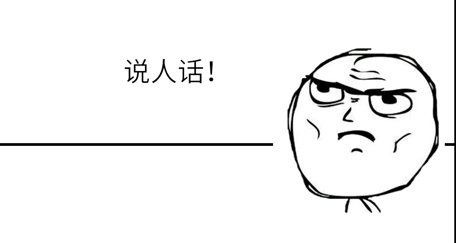
\includegraphics[width=3in]{shuorenhua.png}

\ech
\end{frame}



\begin{frame}
\chtitle{旋量场的量子化}
\bch
人话版本: 对固定$\veck$的$a$粒子和$b$粒子均只存在有限个态$|0\rangle$, $|1\rangle$, ..., $|n_{\max}\rangle$。

\skipline
\skipline
\skipline
这不但是路径积分存在收敛域的必要条件,还顺便使得Hamilton算符的本征值有了下限。
\ech
\end{frame}


\begin{frame}
\chtitle{空穴解释}
\bch
对Hamilton的形式进行物理解释:把$\hatb_{-\veck,s}\bdag_{-\veck,s}$看成能量为$\omega$的粒子的“空穴数”。即最多有$n_{\max}$个空穴,空穴都空为真空(能量最低)。如果进一步要求$\bdag_{-\veck,s}\hatb_{-\veck,s}$是普通的粒子数算符。则有
$$\hatb_{-\veck,s}\bdag_{-\veck,s} + \bdag_{-\veck,s}\hatb_{-\veck,s} = n_{\max}$$ 

由此请证明$n_{\max} = 1$。并进一步证明下列反对易关系:
$$\{\hatb_{-\veck,s},\bdag_{-\veck,s}\} = 1$$

$$\{\hatb_{-\veck,s}, \hatb_{-\veck,s} \} = \{ \bdag_{-\veck,s}, \bdag_{-\veck,s}\} = 0$$

假设理论对于正反粒子是对称的,则对a粒子而言同样有同样的反对易关系。
\ech
\end{frame}


\begin{frame}
\chtitle{守恒量}
\bch
利用反对易关系,我们重新写出守恒量的算符表达式:

Hamilton量为
$$\hat{H}_{\veck,s} =  \omega\left(\adag_{\veck,s}\hata_{\veck,s} + \bdag_{-\veck,s}\hatb_{-\veck,s} -1\right)$$
三维动量为
$$\hat{\mathbf{P}}_{\veck,s} =  \veck\left(\adag_{\veck,s}\hata_{\veck,s} - \bdag_{-\veck,s}\hatb_{-\veck,s} + 1 \right)$$
守恒荷为
$$\hat{Q}_{\veck,s} =  q\left(\adag_{\veck,s}\hata_{\veck,s} - \bdag_{-\veck,s}\hatb_{-\veck,s} + 1 \right)$$

\ech
\end{frame}

\begin{frame}
\chtitle{不同自由度的产生湮灭算符到底该对易还是反对易?}
\bch

因为可观测量都是产生湮灭算符的偶数次,所以这个问题不重要。我们在旋量理论里人为地规定它们反对易。当然,这样可观测量的算符还是对易的。
\ech
\end{frame}

\end{document}

